\documentclass[letterpaper,11pt]{article}

\usepackage[shortlabels]{enumitem}
\usepackage[margin=1in]{geometry}
\usepackage[most]{tcolorbox}
\usepackage{hyperref}

\begin{document}
\title{{\bf Module 4: Research Proposal} }
\author{Name: }

\date{}
\maketitle

\section{Intro}
You have your question and plenty of backup ideas, as well a much better understanding of the field, existing research landscape, and cool directions. Now we're going to figure out exactly how to answer that question. 

We're putting everything together now, and by the end of this worksheet you will have a full blown research proposal that you can continue through I2 (and I hope you all do!), or you will have the experience and skills to thoroughly begin other research avenues. 

I encourage you all to dream about the impacts of your research and to obsessively worry about possible negative side effects. What change do you want to make? How will you get there?

And, as always, you should do this worksheet WITH YOUR TEAM! Look at the sun! It's out there these days! Go meet in the quad or something.

\newline

\section{Research Proposal Template}
For the following sections, if you do not yet have a fully formed answer for the section, note what knowledge you are missing in order to answer the question and how you can find that knowledge!
\subsection{Title and Abstract}
\begin{enumerate}
    \item 
    Provide a concise and descriptive title for your research project proposal. \\
    Write a brief summary of your research proposal, which may include objectives, methods, and expected outcomes.
    \begin{tcolorbox}
TODO: Your answer here
\newline
\newline
\newline
\newline
\newline
\newline
\newline
\newline
\newline
\newline
\newline
\end{tcolorbox}

\subsection{Introduction}
\item 
    Provide background information on the research topic and explain why it is important. \\
    Identify the research problem or question that your proposal aims to address. (This should be easy now) \\
    Discuss the significance and potential impact of your research! \\
\begin{tcolorbox}
TODO: Your answer here
\newline
\newline
\newline
\newline
\newline
\newline
\newline
\newline
\newline
\end{tcolorbox}

\subsection{Literature Review}
\item
Use the literature review you have conducted so far to identify and review relevant literature on your research topic. \\ 
Summarize and analyze the existing knowledge in the field. \\
Identify any gaps or limitations in the current research.
\begin{tcolorbox}
TODO: Your answer here
\newline
\newline
\newline
\newline
\newline
\newline
\newline
\newline
\newline
\end{tcolorbox}

\subsection{Methodology}
\item
    Describe the methods you will use to investigate the research problem or question, and how you expect the end result to look. What are the deliverables from this project? \\ 
    Explain how you will find, create, and/or analyze data, and what tools or techniques you will use. \\ 
    Discuss any potential challenges or limitations in your methodology. \\ 
\begin{tcolorbox}
TODO: Your answer here
\newline
\newline
\newline
\newline
\newline
\newline
\newline
\newline
\newline
\end{tcolorbox}

\subsection{Timeline and Budget}
\item
    Develop a rough timeline for your research project, including key milestones and deadlines.
    Estimate the resources required to complete your research project.
    It might be easiest to draw this out and upload a photo here instead.
\begin{tcolorbox}
TODO: Your answer here
\newline
\newline
\newline
\newline
\newline
\newline
\newline
\newline
\newline
\end{tcolorbox}

\subsection{Conclusion}
\item
    Summarize the key points of your research proposal, focusing on the question, a concise description of how the methodology answers it, and the impacts. \\
\begin{tcolorbox}
TODO: Your answer here
\newline
\newline
\newline
\newline
\newline
\newline
\newline
\newline
\newline
\end{tcolorbox}
\end{enumerate}

\begin{figure}[h]
\caption{This is a photo on Highway 101 going north from San Francisco somewhere. I guess I technically saw the Redwoods too but by the time we got there it was midnight lol. My friend chugged a Monster and drove half the night and I woke up at 5 somewhere on the border of Oregon and California and took over. We had to get back to let his dog out...}
\centering
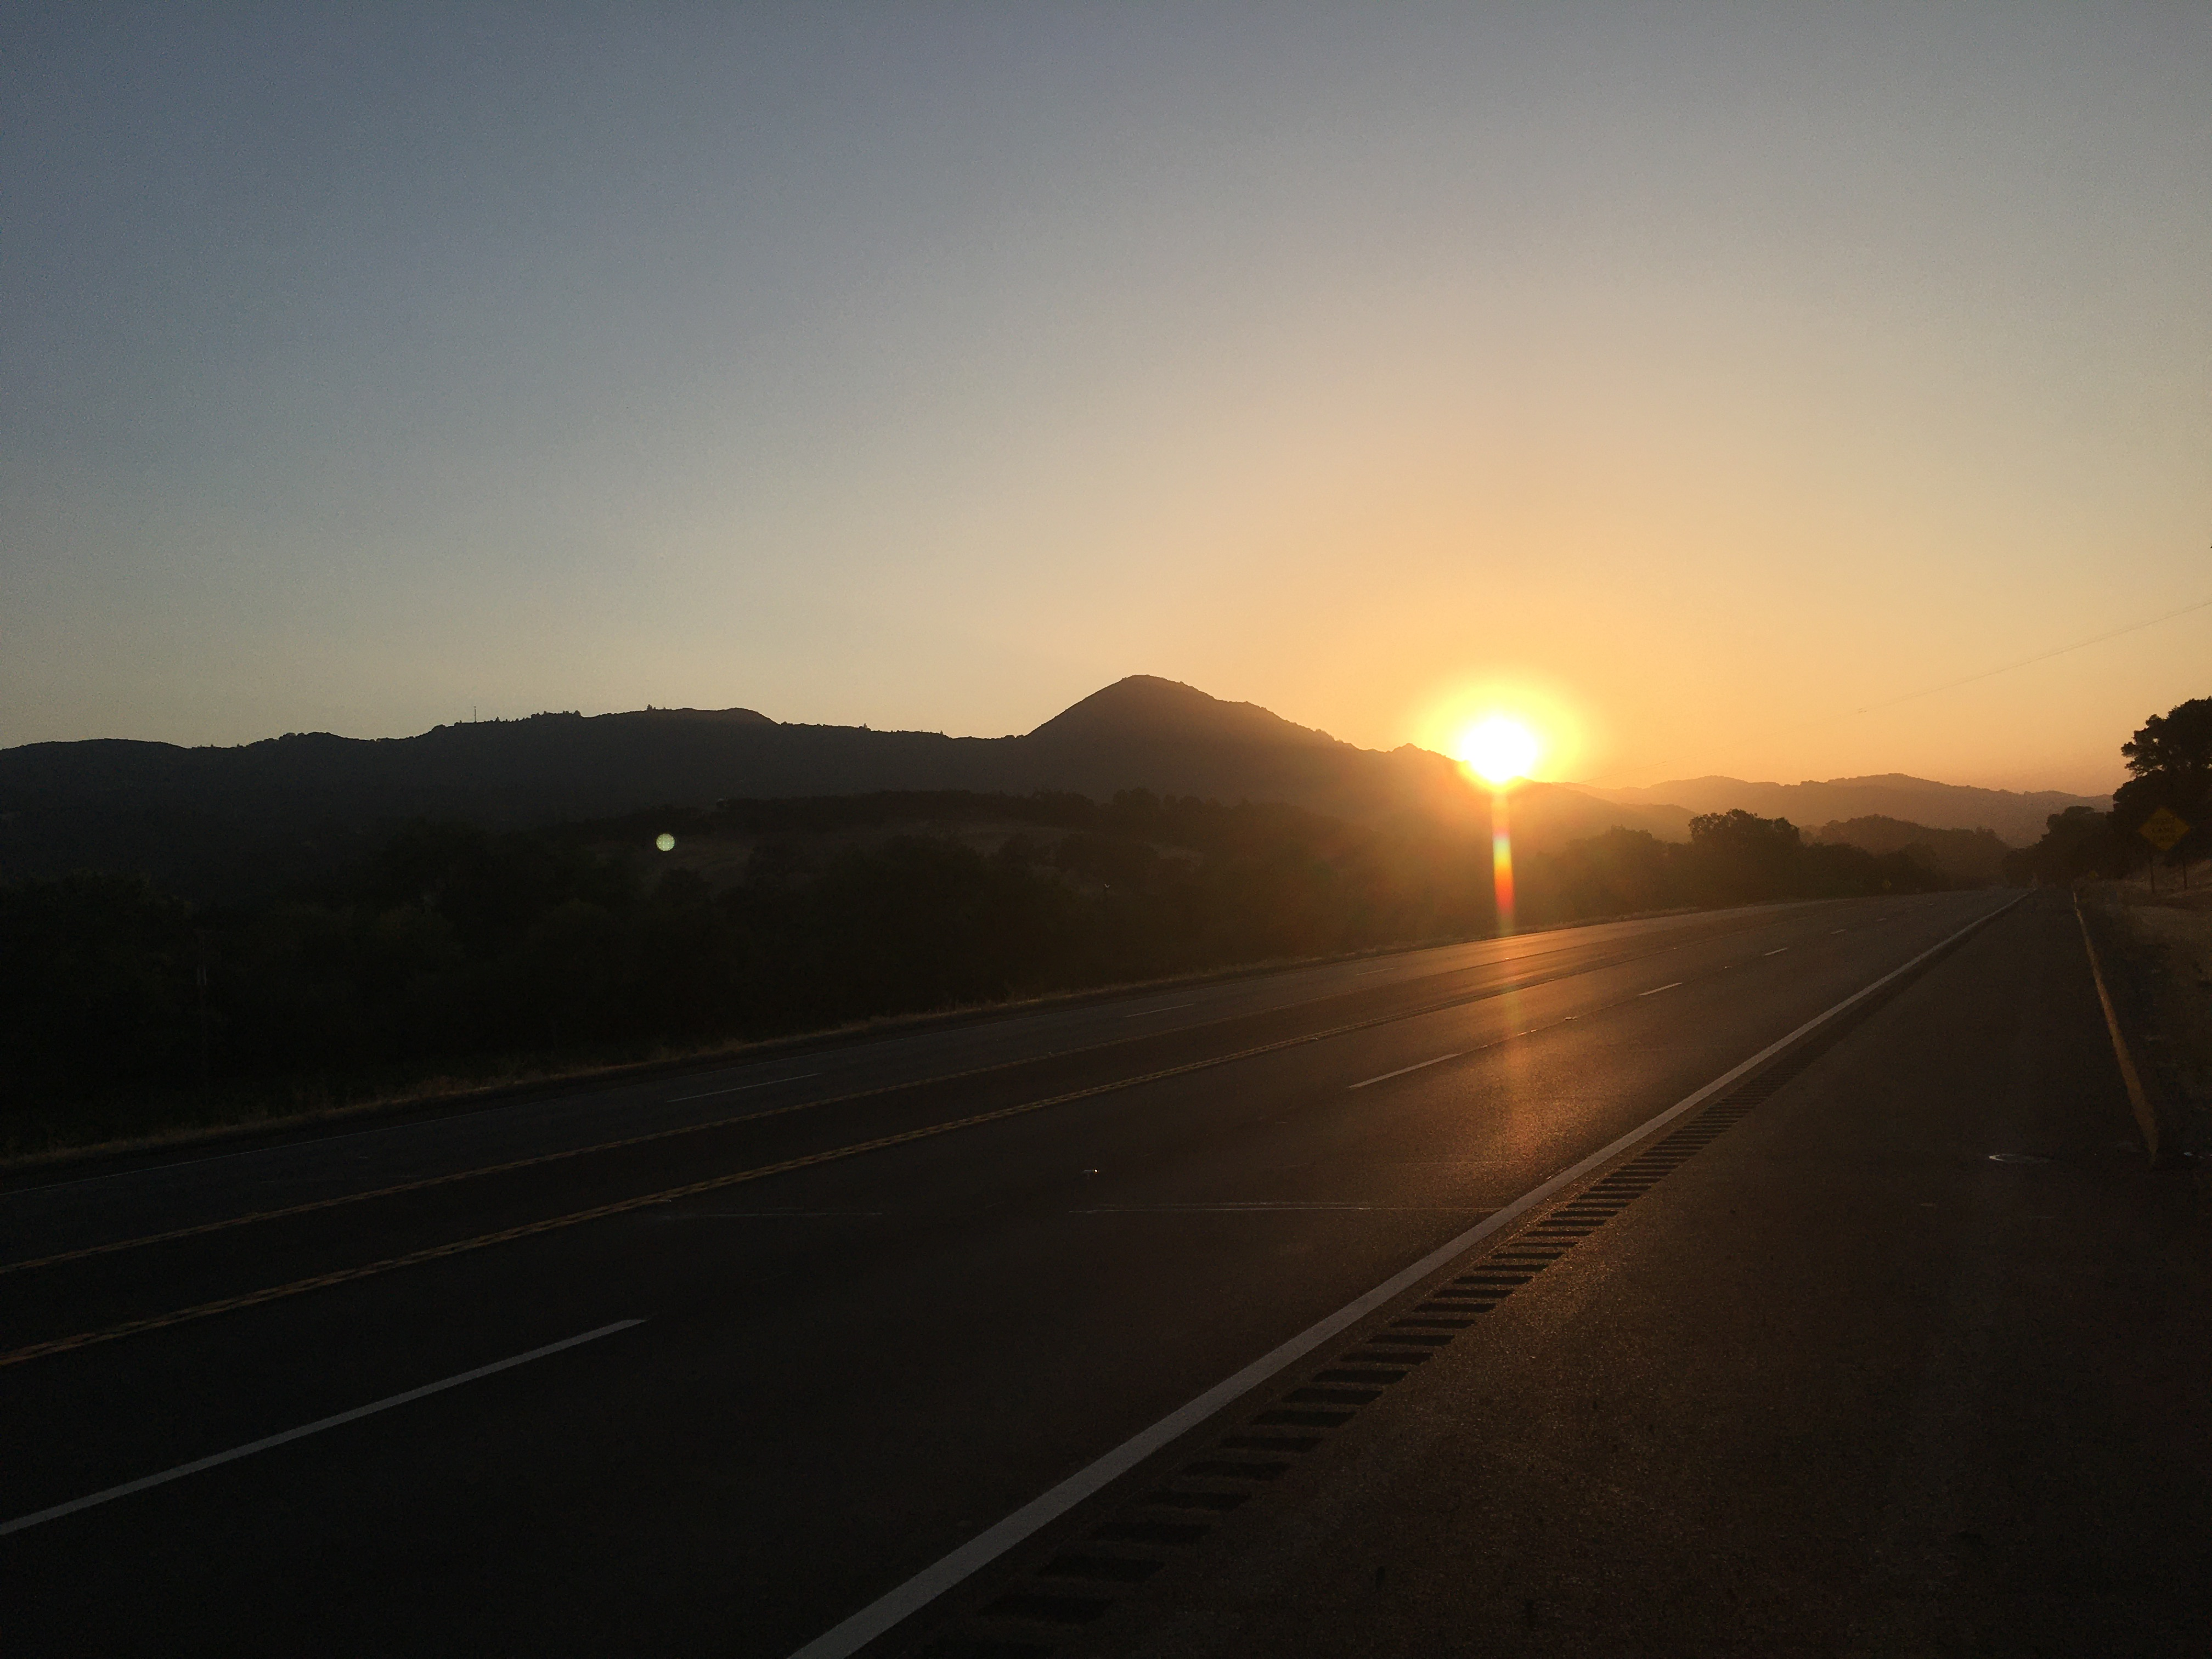
\includegraphics[width=0.5\textwidth]{101.JPG}
\end{figure}

\end{document}
